%*****************************************************************************************
%*********************************** Third Chapter **************************************
%*****************************************************************************************

\chapter{Plasmonic nanostructures}

\graphicspath{{Chapter3/Figures/}}

Surface plasmons are collective electron oscillations at a metallic interface. The form of such oscillations can be found by solving Maxwell's equations, and depends on the experimental geometry. Resonant electron motion causes large electromagnetic field enhancements, while the frequency is very sensitive to the dielectric environment around the metal. In this Chapter Maxwell's equations are solved to find the form of plasmon oscillations at a planar metal-dielectric interface, followed by considerations on how a periodic corrugation of the metal surface affects these solutions. Finally localised surface plasmons on	metal nanoparticles are explored.

\section{Surface plasmon polaritons (SPPs)}
In order to describe the behaviour of electrons in a metal, Maxwell's equations can be used to describe the behaviour of electromagnetic fields:
\begin{subequations}
\label{Maxwell}
\begin{align}
\nabla \cdot \vec{D} &= \rho \label{Maxwell1}\\
\nabla \cdot \vec{B} &= 0 \label{Maxwell2}\\
\nabla \times \vec{E} &= - \frac{\partial \vec{B}}{\partial t} \label{Maxwell3}\\
\nabla \times \vec{H} &= \vec{J} + \frac{\partial \vec{D}}{\partial t} \label{Maxwell4}. 
\end{align}
\end{subequations}
These equations link the fields $\vec{D}$ (dielectric displacement), $\vec{E}$ (electric field), $\vec{H}$ (magnetic field) and $\vec{B}$ (magnetic flux density). The electric charge density is given by $\rho$, and the electric current density by $\vec{J}$. For linear, isotropic and non-magnetic materials we have the relationships
\begin{subequations}
\label{fieldrelations}
\begin{align}
\vec{D} &= \epsilon \epsilon_0 \vec{E} \label{DE}\\
\vec{B} &= \mu \mu_0 \vec{H} \label{BH},
\end{align}
\end{subequations}
where $\epsilon_0, \mu_0$ are the permittivity and permeability of free space respectively, and $\epsilon, \mu$ are the relative permittivity and permeability of the material in question. In the case of a non-magnetic medium $\mu=1$, and the refractive index $n=\sqrt{\epsilon}$.

By combining Eqs.\,\ref{Maxwell3} and \ref{Maxwell4} and assuming a harmonic time dependence to the electric field with frequency $\omega$ such that $\vec{E}(\vec{r},t) = \vec{E}(\vec{r})e^{-i\omega t}$, we find the Helmholtz equation
\begin{equation}
\centering
\nabla^2\vec{E} + k_0^2\epsilon \vec{E} = 0,
\label{Helmholz}
\end{equation}
where $k_0 = \frac{\omega}{c}$ is the wavevector of the wave in vacuum.
\begin{figure}[h!] 
\centering    
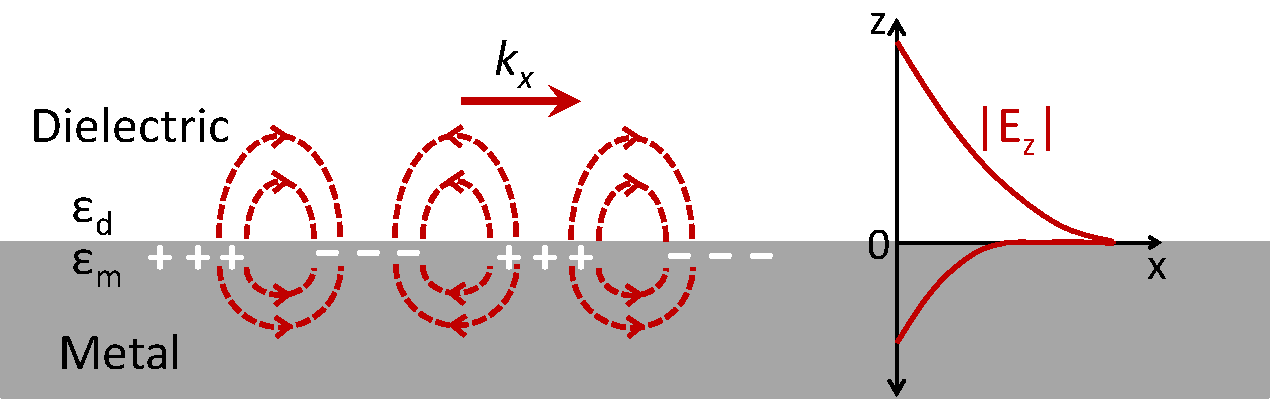
\includegraphics[width=\textwidth]{Fig1}
\caption{Schematic of SPP oscillations at a metal-dielectric surface and the evanescently decaying electric field caused by such plasmons.}
\label{3Fig1}
\end{figure}

Using the geometry of a metal-dielectric interface shown in Fig.\,\ref{3Fig1}, we look for solutions of waves propagation in the $x$ direction but confined to the interface with evanescent decay in the $z$ direction, such that $\vec{E}(x,y,z)=\vec{E}(z) e^{i k_x x}$ where $k_x$ is the propagation constant of the wave. We find one set of solutions that is transverse electric (TE) polarised, with the $\vec{E}$-field component perpendicular to the direction of travel:
\begin{subequations}
\label{TEplasmons}
\begin{align}
H_x &= i \frac{1}{\omega \mu_0} \frac{\partial E_y}{\partial z}\\
H_z &= \frac{k_x}{\omega \mu_0} E_y\\
\frac{\partial^2 E_y}{\partial z^2} &+ (k_0^2 \epsilon_i-k_x^2)E_y = 0 .
\end{align}
\end{subequations}
The subscript $i$ refers to the medium in which the wave is travelling, either $d$ or $m$ for the dielectric and metal respectively. The solutions are waves of the form $e^{i k_x x} e^{k_i z}$. Applying the boundary condition of $E_y$ and $H_x$ continuity across the metal-dielectric interface, we find the condition 
\begin{equation}
\centering
A(k_m+k_d)=0 ,
\label{TEcont}
\end{equation}
where $A$ is the amplitude of wave in the metal halfspace. Since confinement requires Re$(k_m, k_d)>0$, Eq.\,\ref{TEcont} is only fulfilled if $A=0$, i.\,e.\,when no wave can be sustained in the metal. Boundary conditions indicate the wave amplitude of the wave must be 0 in the dielectric as well, thus no SPPs exist in TE polarisation.

The transverse magnetic (TM) polarised solution, with the $\vec{H}$-field component perpendicular to the direction of travel, is:
\begin{subequations}
\label{TMplasmons}
\begin{align}
E_x &= -i \frac{1}{\omega \epsilon_i \epsilon_0} \frac{\partial H_y}{\partial z}\\
E_z &= -\frac{k_x}{\omega \epsilon_i \epsilon_0} H_y\\
\frac{\partial^2 H_y}{\partial z^2} &+ (k_0^2 \epsilon_i-k_x^2)H_y = 0 \label{TMwave}.
\end{align}
\end{subequations}
Here continuity of $H_y$ and $\epsilon_i E_z$ across the interface requires
\begin{equation}
\centering
\frac{k_d}{k_m} = -\frac{\epsilon_d}{\epsilon_m} ,
\label{TMcont}
\end{equation}
so Re[$\epsilon_m$] and $\epsilon_d$ must be of opposite signs, thus SPPs can only be sustained at a metal-insulator interface. Fulfilment of Eq.\,\ref{TMwave} leads to 
\begin{subequations}
\label{k_relations}
\begin{align}
k_m^2 &= k_x^2-k_0^2\epsilon_m\\
k_d^2 &= k_x^2-k_0^2\epsilon_d ,
\end{align}
\end{subequations}
and combining this with Eq.\,\ref{TMcont} produces
\begin{equation}
\centering
k_x = k_0\sqrt{\frac{\epsilon_m \epsilon_d}{\epsilon_m + \epsilon_d}} ,
\label{SPPdispersion}
\end{equation}
the dispersion relation of an SPP on a metal-dielectric interface. Fig.\,\ref{3Fig2}(a) shows the calculated dispersion for Ag-air SPPs, using a free electron gas model where there is no damping in the metal \cite{Zeman1987}, i.\,e.\,Im($\epsilon_m)=0$. The SPP dispersion can be separated into three regions: at frequencies above the plasma frequency of the electron gas $\omega_p$ we have the transparent region ($k_x, k_i$ real) where radiation can penetrate into the metal and excite volume plasmon polaritons. At frequencies below the surface plasmon frequency $\omega_{sp}$ we have bound surface modes ($k_x$ real, $k_i$ imaginary). In the limit $k_x\rightarrow \infty$ plasmons become stationary surface plasmons, where the resonance frequency $\omega_{sp} = \frac{\omega_p}{1+\epsilon_d}$ and $\epsilon_m+\epsilon_d=0$. For $\omega_{sp}<\omega<\omega_p$ no propagating modes exist ($k_x$ imaginary). If damping is included in the metal dielectric function \cite{Johnson1972}, then quasi-bound modes can exist in this intermediate region [Fig.\,\ref{3Fig2}(b)]. Note damping introduces a finite maximum $k_x$ for SPPs, leading to a finite propagation length $L_x = \frac{1}{2\textnormal{Im}(k_x)}$, typically on the order $10-100\,$\textmu m at visible wavelengths for Au/Ag \cite{Maier2007}. The limit in $k_x$ also produces an upper limit in $k_i$ [Eq.\,\ref{k_relations}], thus limiting the skin depth $L_z = \frac{1}{\textnormal{Im}(k_i)}$ to $\sim10$\,nm in metals. 
\begin{figure}[h!] 
\centering    
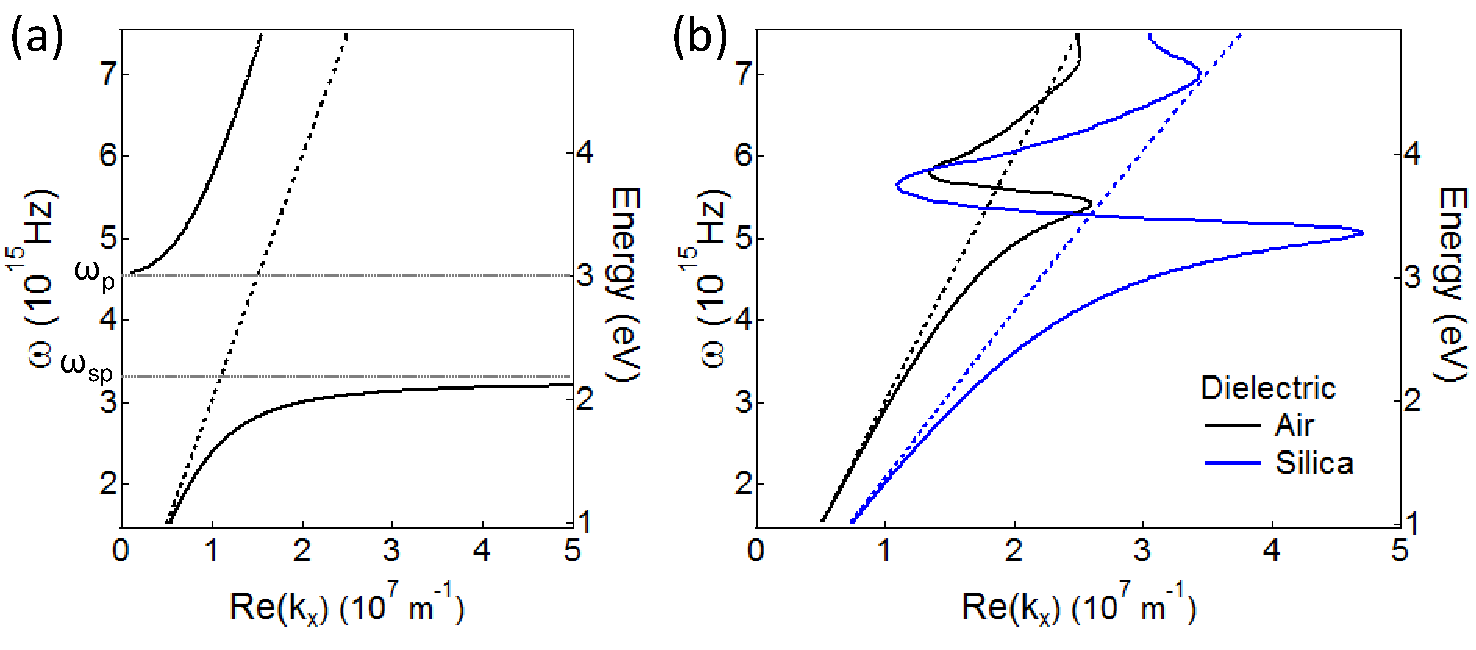
\includegraphics[width=\textwidth]{Fig2}
\caption{Dispersion of SPPs at an (a) Ag (free electron gas)-air \cite{Zeman1987} and (b) Ag (with absorption)-air/silica interface \cite{Johnson1972} (solid lines). Light lines in the dielectric are shown by dashed lines.}
\label{3Fig2}
\end{figure}


\section{Plasmonic gratings}
\label{sec:plasmonicgratings}
\begin{figure}[h!]
\centering
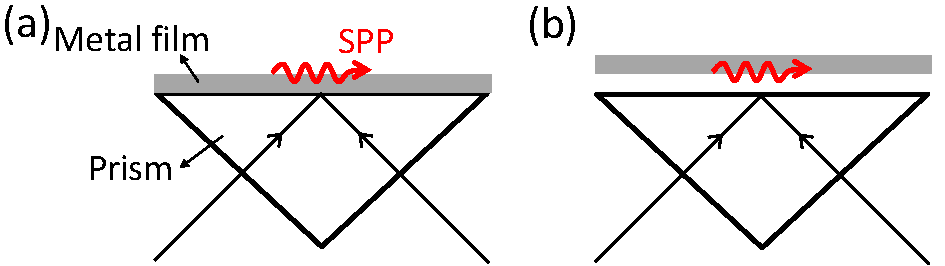
\includegraphics[width=0.8\textwidth]{PrismCoupling}
\caption{Prism coupling to surface plasmon polaritons in the (a) Kretschmann and (b) Otto configurations.}
\label{PrismCoupling}
\end{figure}
The momentum mismatch between SPPs and photons in a dielectric [Fig.\,\ref{3Fig2}] means that it is not possible to directly optically excite SPPs. Instead we must use a phase matching technique, for example prism or grating coupling. In prism coupling a three-layer system is employed either in the Kretschmann or Otto configurations [Fig.\,\ref{PrismCoupling}], in both cases the evanescent field of photons in a higher refractive index material has sufficient momentum to excite SPPs on the interface between a metal and lower refractive index material. In grating coupling, momenta $\hbar\frac{2\pi}{D}m = \hbar G_m$ (integer $m$) can be provided by standing waves set up in a structure with periodicity $D$, thereby allowing photons to couple to SPPs. However in a periodic plasmonic nanostructure SPPs can interact with diffracted photons to produce complex optical spectra, which will be discussed below.

\subsection{First order modes}
\begin{figure}[h!p] 
\centering    
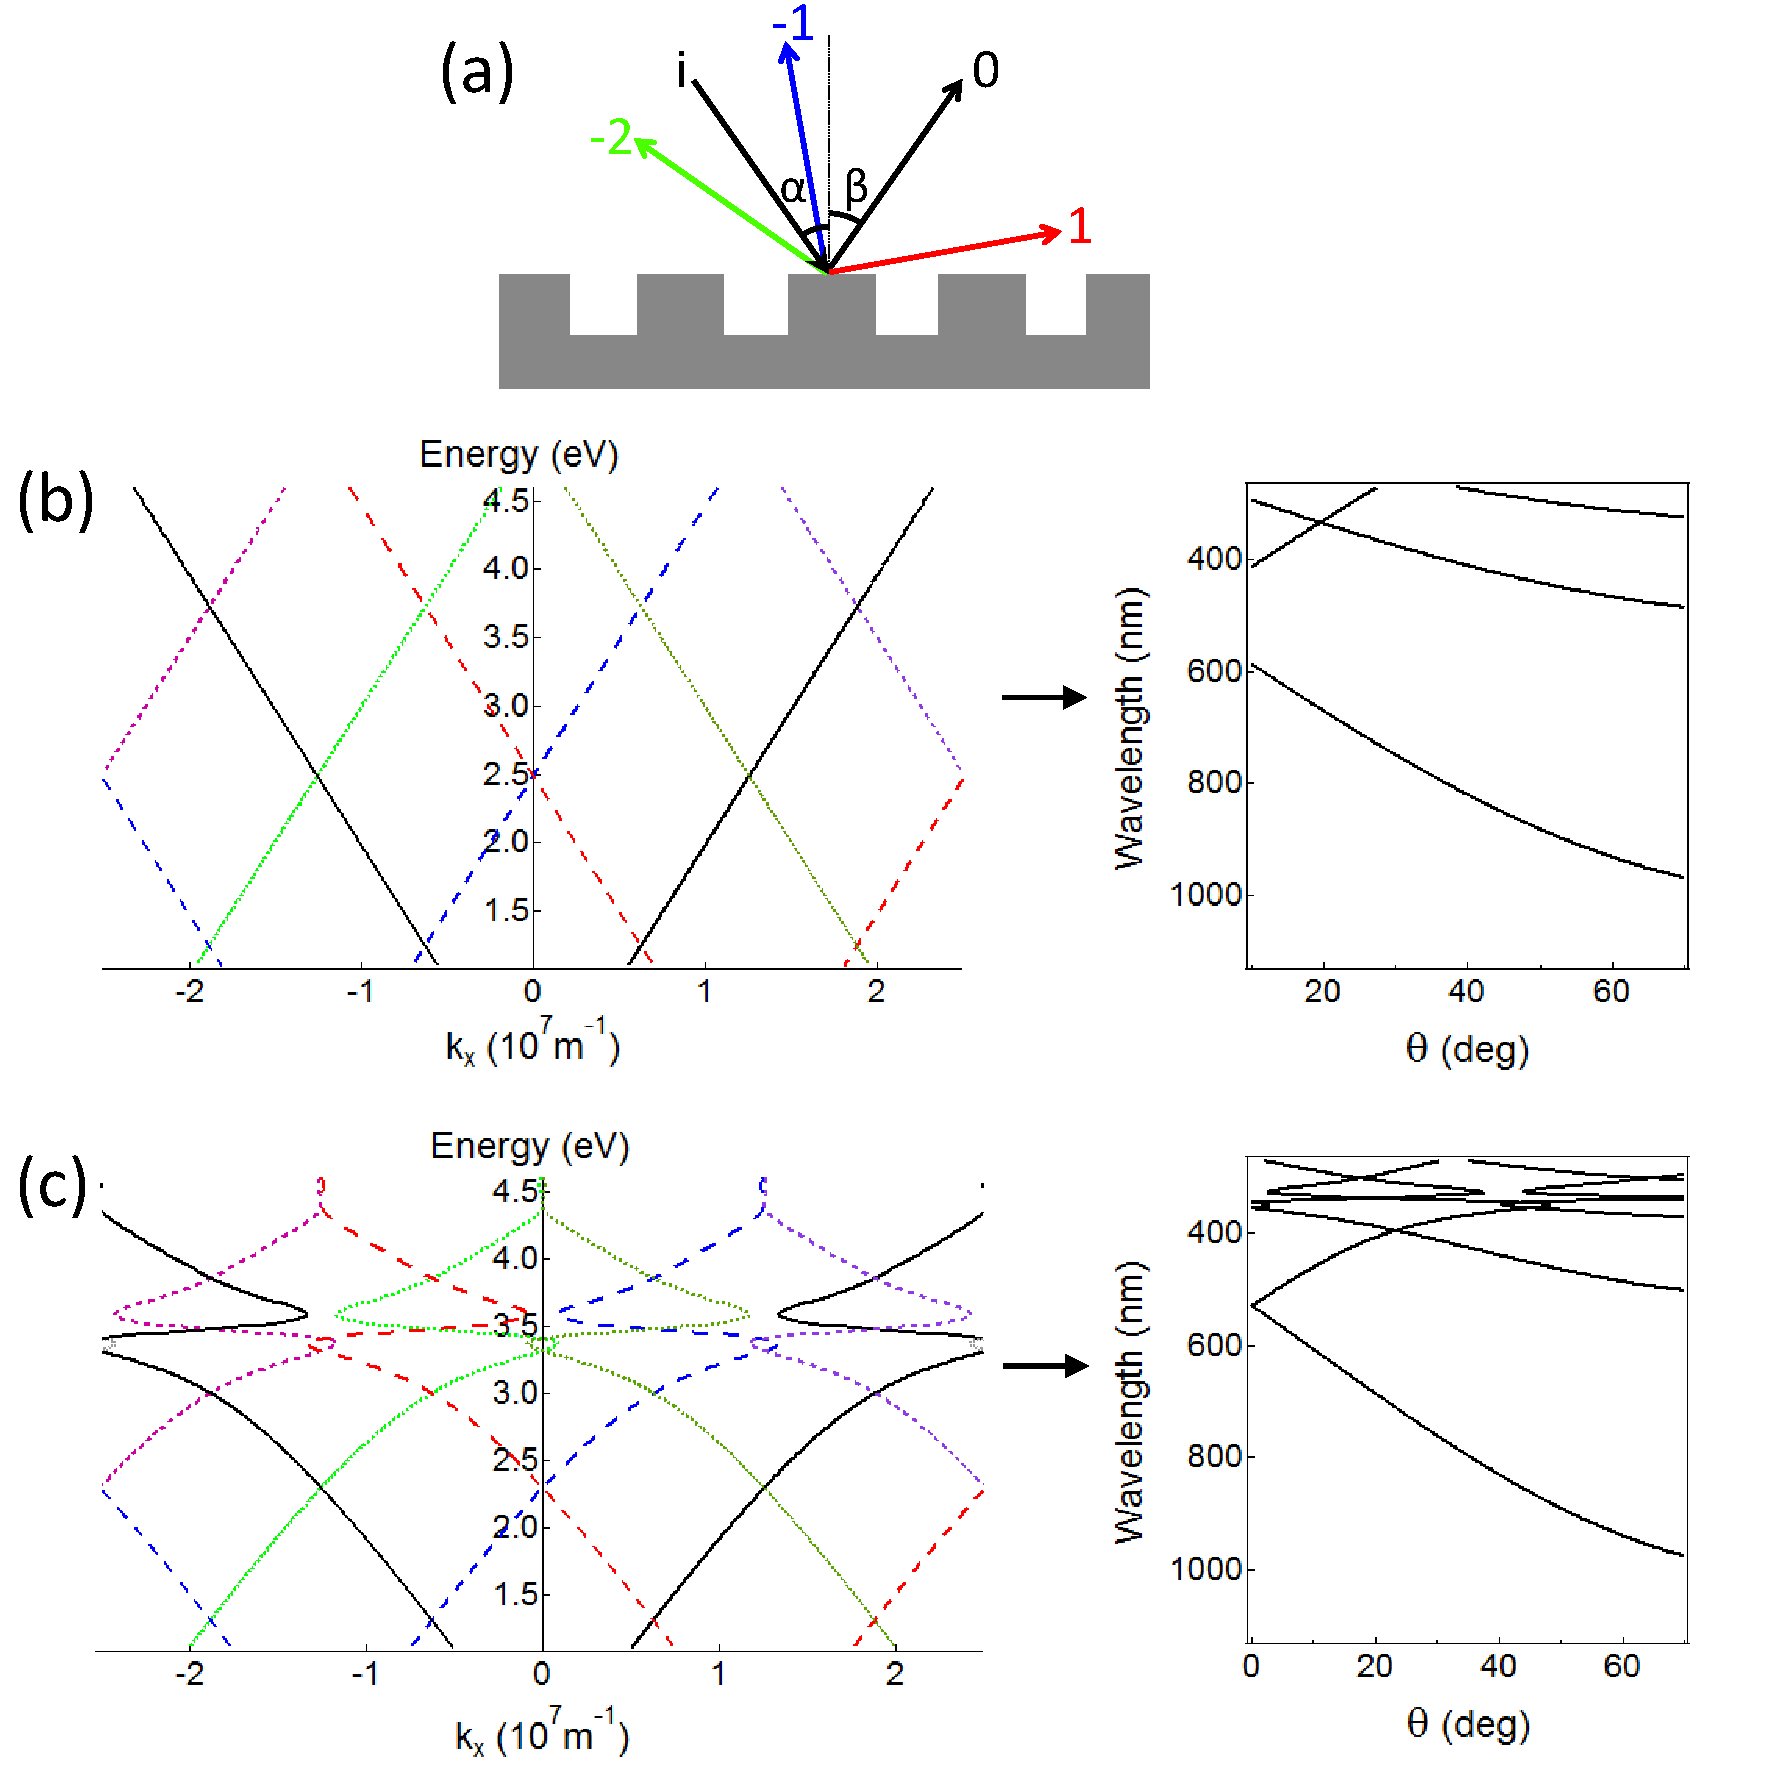
\includegraphics[width=\textwidth]{Fig3}
\caption{(a) Diffraction from a 1D grating, illustrating the incident light $i$ and diffracted orders $n$. Dispersion (left) and mode positions in specular reflection as a function of incidence angle $\theta$ (right) for (b) photonic and (c) plasmonic first order modes of a $D=500$\,nm Ag grating in air at $\phi=0^{\circ}$.}
\label{3Fig3}
\end{figure}
Using Huygens' construction and considering each point on the grating as a wave scatterer, we reach the well-known grating equation for constructive interference
\begin{equation}
\centering
D(\sin\alpha-\sin\beta) = n\lambda ,
\label{GratingEq}
\end{equation}
where $\alpha$ is the angle of incidence and $\beta$ the diffracted angle with respect to the grating normal, $\lambda$ is the wavelength and $n$ the order of the diffracted light [Fig.\,\ref{3Fig3}(a)]. From here we will only consider the zeroth diffraction order (specular reflection) with incidence angle $\theta$ and azimuthal angle $\phi$. In the first order approximation we assume no interactions between diffracted fields, and can distinguish between two types of gratings modes: `photonic' modes caused purely by the interference of light, and `plasmonic' modes where SPPs are excited on the surface of the grating. We can find the dispersion of such grating modes by considering momentum and energy conservation of incoming/outgoing photons, and find
\begin{equation}
\centering
k = k_i^2\sin^2\theta+G_m^2\pm2k_iG_m\sin\theta\cos\phi ,
\label{GratingDisp}
\end{equation}
where the $m$ labels the grating vector $G_m$ needed for momentum matching. Here
\begin{subequations}
\label{kmodes}
\begin{align}
\centering
k_i &= \frac{\omega}{c}\sqrt{\epsilon_d}& \\
k&=\frac{\omega}{c}& \textnormal{for photons} \label{kphot} \\
k &= \frac{\omega}{c}\sqrt{\frac{\epsilon_m\epsilon_d}{\epsilon_m+\epsilon_d}}& \textnormal{for SPPs .} \label{kspp}
\end{align}
\end{subequations}
The dielectric function of the material coating the grating is given by $\epsilon_d$. In this case the grating can be thought of as a 1D photonic crystal, and the photon and SPP dispersions are displaced by multiples of the grating vector $G_1$ [Fig.\,\ref{3Fig3}(b,c)]. Different SPP modes on the metal surface can strongly couple and create anticrossings in spectra \cite{Chen1983}.



\subsection{Grating anomalies}

Anomalies are sharp changes in the response of a grating, and first observed by Wood, who noted ``that under certain conditions the drop from maximum illumination to minimum...occurred within a range of wave-lengths not greater than the distance between sodium lines" \cite{Wood1902}. So called Wood's anomalies are second order effects, where interactions between diffracted fields are taken into account. In plasmonic gratings we can further separate this phenomenon into threshold (sharp changes in intensity) and resonance (dip in intensity at higher wavelength) anomalies [Fig.\,\ref{3Fig4}].
\begin{figure}[h!] 
\centering    
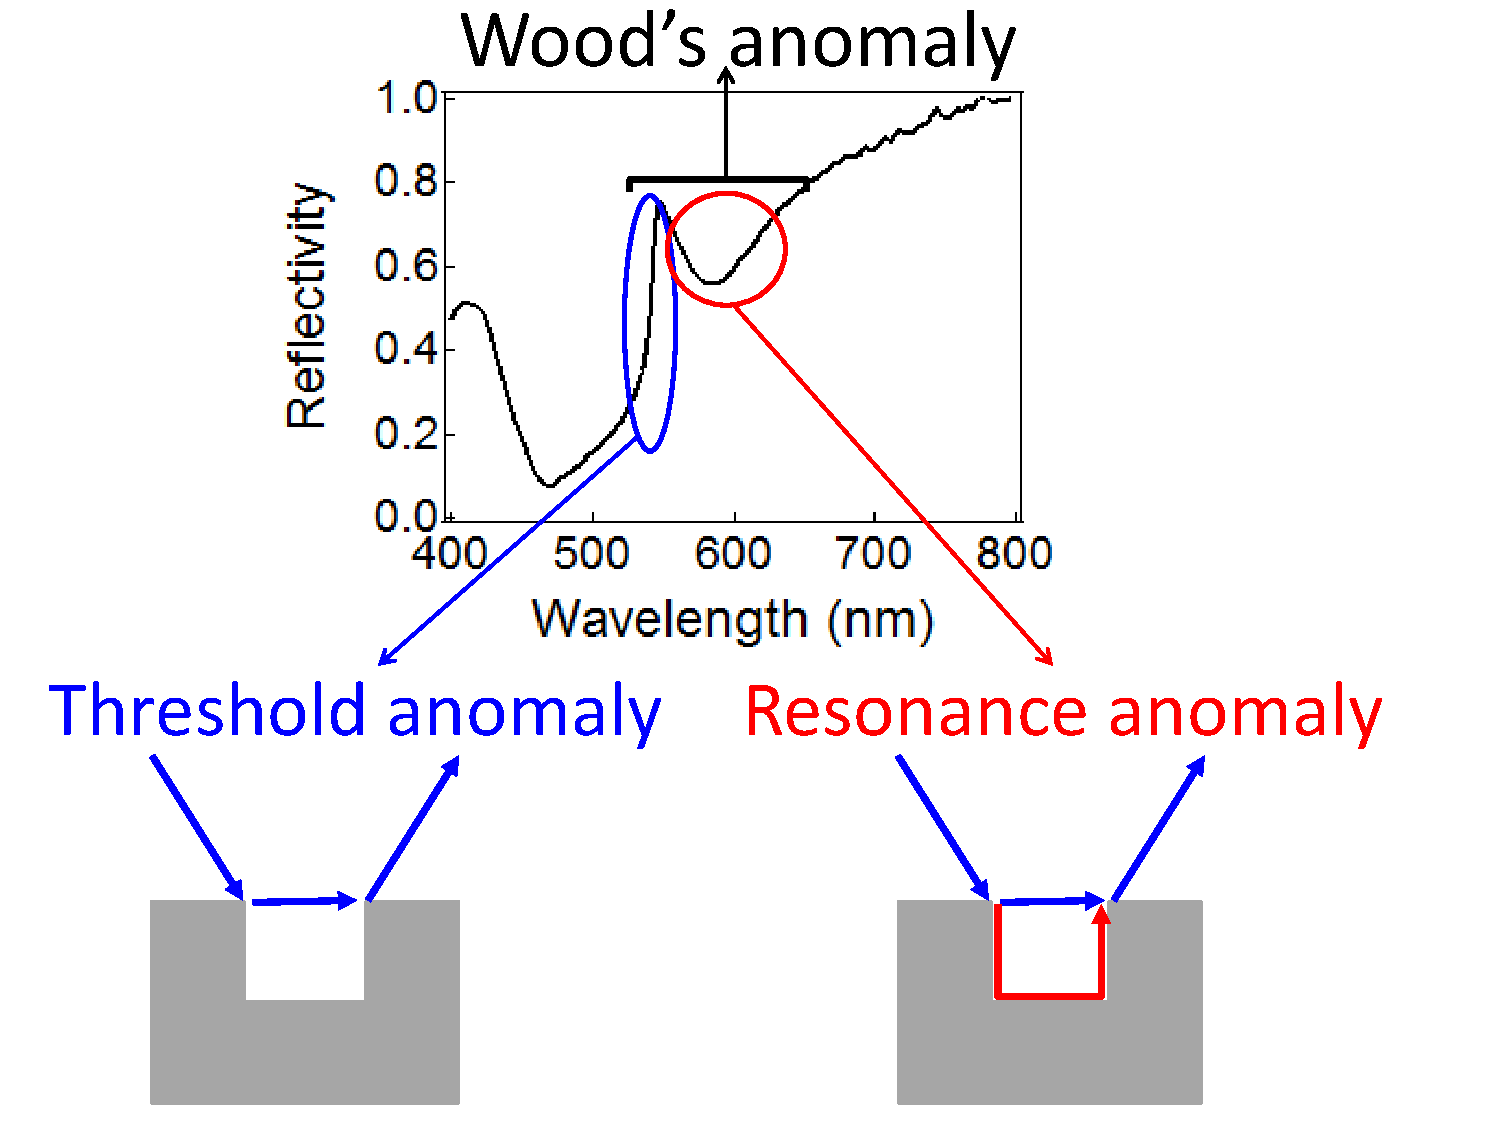
\includegraphics[width=0.75\textwidth]{Fig4}
\caption{Wood's anomaly in the TM-polarised specular reflectivity of a $D=417$\,nm Ag grating in air. Illustrations of the threshold and resonance anomaly processes are shown (bottom).}
\label{3Fig4}
\end{figure}

The threshold anomaly is a photonic effect, and comes about when an order is diffracted along the surface of the grating ($\beta=90^{\circ}$). If the order becomes evanescent then the energy available will be redistributed to other diffractive orders. Thus this `passing' order on the edge between diffraction ($\beta<90^{\circ}$) and evanescence ($\beta>90^{\circ}$) causes a sharp change in the diffraction intensity of other orders, and are observed in the positions of first order photonic modes [Eq.\,\ref{GratingDisp}]. Threshold anomalies can be observed in both polarisations, but generally anomaly strength (i.\,e.\,the difference between maximum and minimum intensity) is smaller in TE polarisation, particularly in metals. In this case the $\vec{E}$-field is parallel to grating lines and cannot be sustained, leading to less energy redistribution, and a reduction in the effect. Threshold anomalies can be observed in both reflection and transmission gratings, and are responsible for the extraordinary transmission seen in 1D and 2D hole arrays \cite{Fano1941, Hessel1965, Lee2005, Lochbihler1994, Ritchie1968, Treacy2002, Watts1997}.
\begin{figure}[h!] 
\centering    
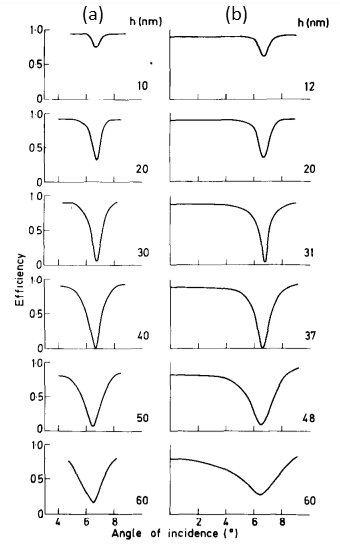
\includegraphics[width=0.6\textwidth]{Fig5}
\caption{(a) Electromagnetic theory modelling and (b) experimental dependence of the resonance anomaly on the grating depth $h$ for $D=556$\,nm sinusoidal Au grating at $\lambda=647$\,nm \cite{Hutley1976}. }
\label{3Fig5}
\end{figure}

The resonance anomaly is a plasmonic effect, and comes from an interaction between diffracted light and excited surface waves on the grating. The addition of the SPP oscillator and background photonic diffraction produces a Fano resonance, the asymmetric lineshape in Fig.\,\ref{3Fig4}. Resonance anomalies can only be observed in geometries where SPPs can be excited, e.\,g.\,TM polarisation $\phi=0^{\circ}$, TE polarisation $\phi=90^{\circ}$. The dip position and linewidth depend on the nature of the SPP and is sensitive to the grating profile and surface roughness [Fig.\,\ref{3Fig5}]. Therefore we cannot use analytical equations to make predictions about the positions of resonance anomalies, instead we need to use electromagnetic theory to model the grating \cite{Hutley1982, Loewen1997}. In the same way, coatings on gratings affect the electromagnetic field near the surface and can change the position and strength of anomalies, particularly resonance anomalies. In addition, modes excited in the coating material can change the $\vec{E}$-field polarisation and excite anomalies in previously forbidden geometries \cite{Hutley1982, Loewen1997}.



\subsection{Localised and guided modes}
\label{sec:channel}
Gratings can also give rise to optical modes that do not rely on diffraction. In particular the grating slits are independent open electromagnetic waveguides that can sustain TE and TM modes. For example, the dispersion of a TE$_{\mu\nu}$ mode is \cite{Jackson1999}
\begin{equation}
\centering
\frac{\omega^2}{c^2}(n_{\mathit{eff}}^2-\sin^2\theta) = \pi^2\left(\frac{\mu^2}{a_{\mathit{eff}}^2}+\frac{\nu^2}{b_{\mathit{eff}}^2}\right) ,
\label{waveguide}
\end{equation}
where $n_{\mathit{eff}}$ is the effective refractive index experienced by the mode in the grating slit, $a_{\mathit{eff}}$ the effective cavity width and $b_{\mathit{eff}}$ the effective cavity height, and $\mu, \nu$ are indices used to label the waveguide mode. Due to the penetration of electromagnetic fields in metals, $a_{\mathit{eff}}$ is not the same as the geometric width of the grating slit, and particularly if there is a coating on the metal then $a_{\mathit{eff}}$ and $b_{\mathit{eff}}$ both have some dependence on $n_{\mathit{eff}}$. 

If SPPs are excited, then grating slits can be thought of as a metal/insulator/metal waveguide. SPPs travelling on slit edges can interact to form symmetric and antisymmetric combinations, particularly if the slit is narrow \cite{Maier2007}. For rectangular slits, often known as trench waveguides, the highest $\vec{E}$-field intensity is at the top corners of slits and thus extends outside the groove [Fig.\,\ref{3Fig6}(a), right] \cite{Bozhevolnyi2005, Srivastava2009, Chattopadhyay2012}. For V-shaped slits, the gradual change in width leads to multiple reflections and localisation of the $\vec{E}$-field at the bottom of the grooves (adiabatic nanofocusing) [Fig.\,\ref{3Fig6}(a), left] \cite{Bozhevolnyi2005, Srivastava2009, Novikov2002, Kuttge2009, Sondergaard2012}. These modes are called channel plasmon polaritons (CPPs) and can be observed in near-field optical microscopy [Fig.\,\ref{3Fig6}(b)]. Due to their localised nature, CPPs can be distinguished from diffractive grating modes by their relatively flat dispersions.
\begin{figure}[h!] 
\centering    
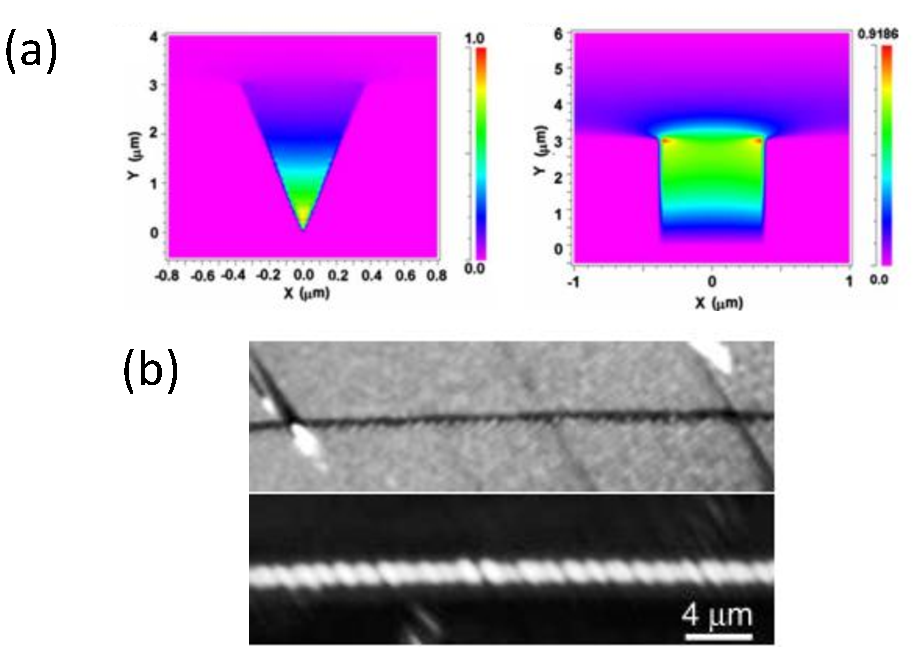
\includegraphics[width=0.9\textwidth]{Fig6}
\caption{(a) $\vec{E}$-field profiles of channel plasmon polariton modes in a V-shaped (left) and trench (right) Au groove, with width 3.75\,\textmu m and depth 3\,\textmu m filled with air \cite{Srivastava2009}. (b) Topographical (top) and near-field optical images (bottom) for V-shaped Au slit with width 0.6\,\textmu m and depth 1\,\textmu m at $\lambda=1440$\,nm. Interference can be seen in the near-field image as a result of interference with scattered light \cite{Bozhevolnyi2005}.}
\label{3Fig6}
\end{figure} 

\begin{figure}[h!] 
\centering    
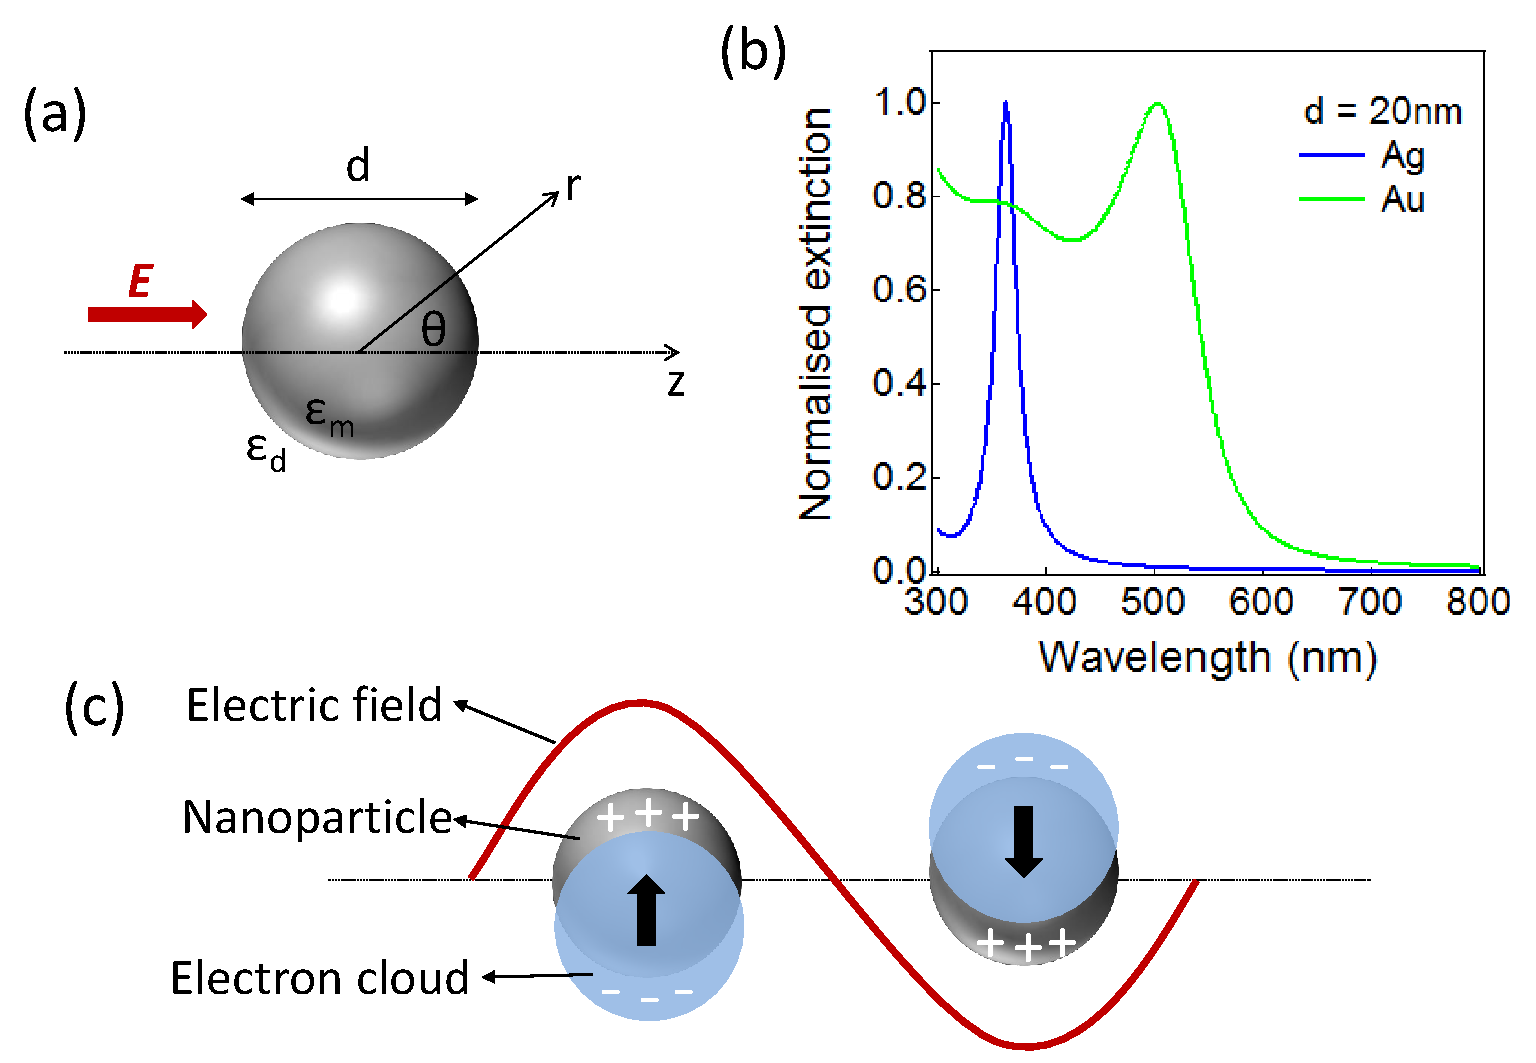
\includegraphics[width=\textwidth]{Fig7}
\caption{(a) Geometry used to calculate the localised surface plasmon resonance of a homogeneous metal sphere with diameter $d$ placed inside an electrostatic $\vec{E}$-field. (b) Normalised extinction spectra for $d=20$\,nm Ag/Au NPs in air. (c) Schematic of dipolar electron oscillations in NPs driven by an electric field. (d) Time averaged $\vec{E}$-field intensity of the dipolar localised surface plasmon mode of a 20\,nm Ag nanoparticle.}
\label{3Fig7}
\end{figure} 
\section{Localised surface plasmons (LSPs)}
\subsection{Quasi-static approximation}

For a spherical nanoparticle (NP) whose diameter $d\ll\lambda$, the phase of the $\vec{E}$-field is approximately constant across the particle and we can solve the simplified problem of a sphere in an electrostatic field, then include the harmonic time dependence as a last step. The geometry is shown in Fig.\,\ref{3Fig7}(a), with a homogeneous metal particle (dielectric function $\epsilon_m$) of diameter $d$ at the origin inside a dielectric medium $\epsilon_d$, and $\vec{E} = E_0\vec{z}$. Solving the Laplace equation for the potential $\Phi$ ($\vec{E} = -\nabla\Phi$), we find
\begin{subequations}
\label{NPlaplace}
\begin{align}
\Phi_{in} &= -\frac{3\epsilon_d}{\epsilon_m+2\epsilon_d}E_0r\cos\theta \label{PhiIn}\\
\Phi_{out} &= -E_0r\cos\theta+\frac{\epsilon_m-\epsilon_d}{\epsilon_m+2\epsilon_d}E_0\left(\frac{d}{2}\right)^3\frac{\cos\theta}{r^2} \label{PhiOut}
\end{align}
\end{subequations}
at a distance $r$ from the centre of the sphere, where $\Phi_{in}$ and $\Phi_{out}$ represent the potentials inside and outside the sphere respectively. From Eq.\,\ref{PhiIn} we can see that the potential and electric field is enhanced at the NP surface by factor of $\frac{3\epsilon_d}{\epsilon_m+2\epsilon_d}$ as a result of the induced surface charges [Fig.\,\ref{3Fig7}(c)]. This effect also appears in Eq.\,\ref{PhiOut}, which is the superposition of the applied field $E_0$ and an induced dipole in the NP with dipole moment $\vec{p}$ and polarisability $\alpha$, such that
\begin{subequations}
\label{NPdipole}
\begin{align}
\vec{p} &=4\pi\epsilon_0\epsilon_d\left(\frac{d}{2}\right)^3\frac{\epsilon_m-\epsilon_d}{\epsilon_m+2\epsilon_d}\vec{E} \label{NPmoment}\\
\alpha &= 4\pi\left(\frac{d}{2}\right)^3\frac{\epsilon_m-\epsilon_d}{\epsilon_m+2\epsilon_d} \label{NPpolarisability} .
\end{align}
\end{subequations}
A resonance in $\alpha$ is achieved when 
\begin{equation}
\centering
\epsilon_m(\omega) = -2\epsilon_d(\omega) ,
\label{Frolich}
\end{equation}
known as the Fr\"{o}lich condition, and provides the resonance frequency of the dipolar LSP for a metallic NP. For a free electron gas in air, this condition is achieved at $\omega = \frac{\omega_p}{\sqrt{3}}$, but will depend on both $\epsilon_m$ and $\epsilon_d$. For this reason the LSP resonance of Ag NPs is at a higher frequency than Au NPs with the same $d$ [Fig.\,\ref{3Fig7}(b)]. Note the asymmetric shape of the Au extinction peak due to the onset of interband transitions. The harmonically oscillating $\vec{E}$-field acts to drive electron oscillations in the NP, and causes a large field enhancement in the vicinity of the particle in the same way as an SPP [Fig.\,\ref{3Fig7}(d)]. For NP arrays, if particles are separated by $\gtrsim2d$ then LSP fields do not interact \cite{Rechberger2003}.
\begin{figure}[h!] 
\centering    
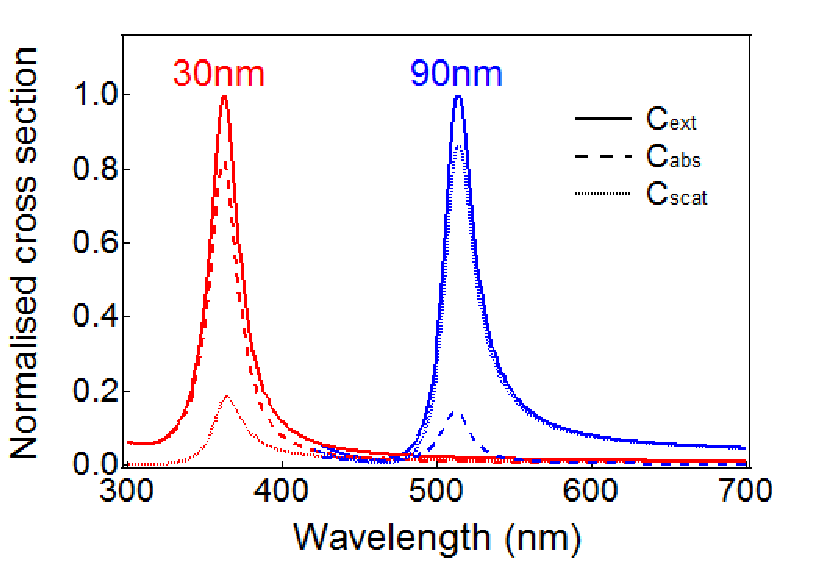
\includegraphics[width=0.7\textwidth]{Fig8}
\caption{Normalise absorption (dashed lines), scattering (dotted lines) and extinction (solid lines) cross sections for $d=30$, 90\,nm Ag nanoparticles at $\lambda=500$\,nm in air according to Eq.\,\ref{NPcrossSections}. The $d=90$\,nm data has been shifted for clarity.}
\label{3Fig8}
\end{figure}

The oscillating NP dipole leads to radiation, which can be seen as scattering of light from the NP. The scattering ($C_{\mathit{scat}}$) and absorption ($C_{\mathit{abs}}$) cross sections of the particle are given by
\begin{subequations}
\label{NPcrossSections}
\begin{align}
C_{\mathit{scat}} &= \frac{k^4}{6\pi}|\alpha|^2 = \frac{8\pi}{3}k^4\left(\frac{d}{2}\right)^6 \left|\frac{\epsilon_m-\epsilon_d}{\epsilon_m+2\epsilon_d}\right|^2 \label{Scat}\\
C_{\mathit{abs}} &= k\textrm{Im}[\alpha] = 4\pik\left(\frac{d}{2}\right)^3\textrm{Im}\left[\frac{\epsilon_m-\epsilon_d}{\epsilon_m+2\epsilon_d}\right] \label{abs} ,
\end{align}
\end{subequations}
and we define extinction $C_{\mathit{ext}} = C_{\mathit{scat}}+C_{\mathit{abs}}$. The resonance in $\alpha$ gives rise to a maximum in the optical response of the NP. For very small NPs absorption dominates over scattering due to its $d^3$ dependence, for example for $d=30$\,nm Ag NPs the extinction is almost entirely due to absorption, while the reverse is true for $d=90$\,nm [Fig.\,\ref{3Fig8}].

\begin{figure}[h!] 
\centering    
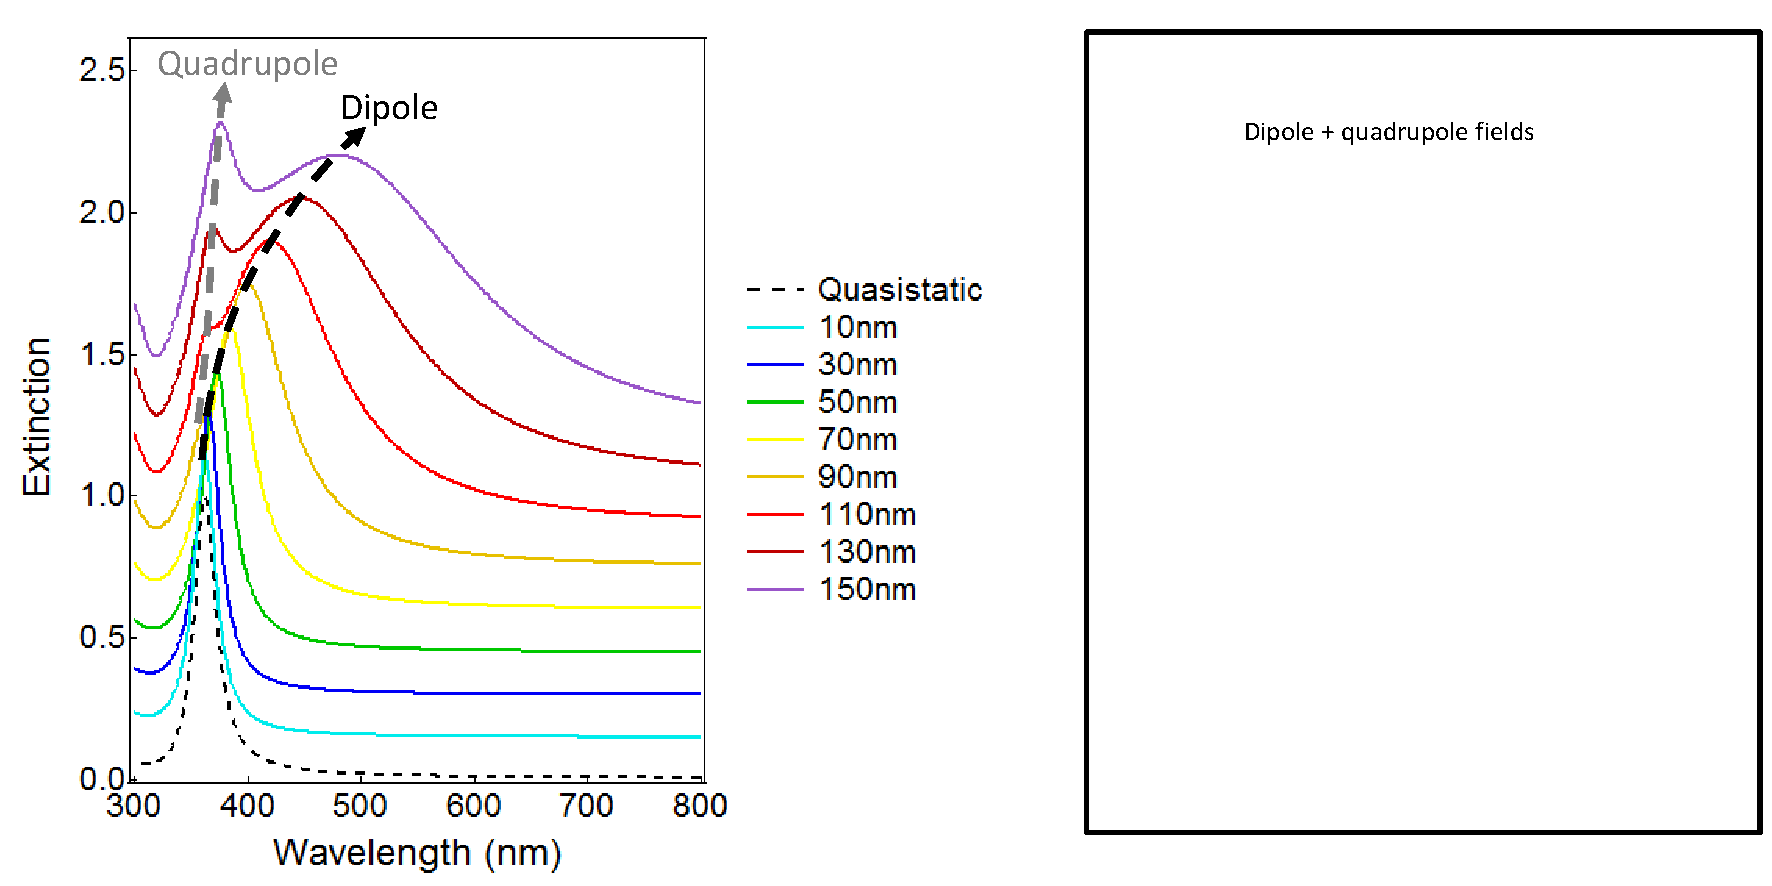
\includegraphics[width=0.8\textwidth]{Fig9}
\caption{Calculated extinction spectra for Ag nanoparticles in air using Mie theory, normalised to the dipole maximum and offset for clarity. The quasi-static approximation resonance is added for comparison.}
\label{3Fig9}
\end{figure}

\begin{figure}[h!] 
\centering    
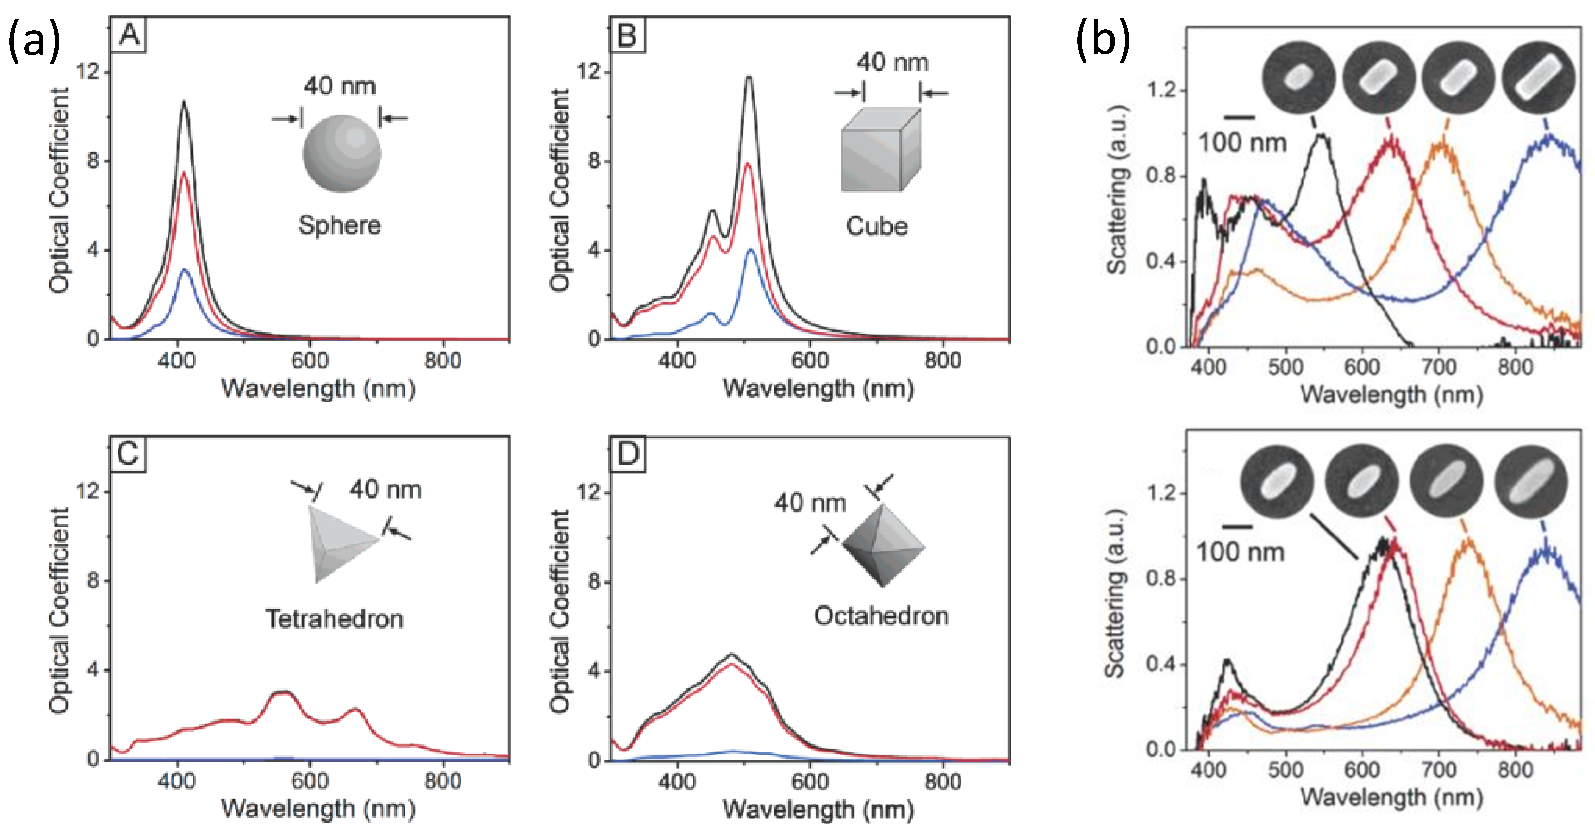
\includegraphics[width=\textwidth]{Fig10}
\caption{(a) Discrete dipole approximation calculations of the extinction (black), absorption (red) and scattering (blue) of Ag nanoparticles with the geometries shown \cite{Wiley2006}. (b) SEM images and normalised scattering spectra of individual Ag nanobar (left) and nanorice (right) structures \cite{Wiley2007}.}
\label{3Fig10}
\end{figure}
\subsection{Size and shape effects}
The quasi-static approximation models the NP as an electric dipole whose resonance frequency depends purely on the relative dielectric functions of the metal and surrounding medium. The underlying assumption that the phase of the $\vec{E}$-field across the particle is constant is only true for very small particles, and works well for $d<50$\,nm Ag particles [Fig.\,\ref{3Fig9}]. For larger particles an electrodynamic model must be used, for example Mie theory, where the electromagnetic field is separated into subfields made of infinite series of of partial waves with spherical polar geometry. Applications of boundary conditions and Maxwell's equations leads to a set of differential equations that can be solved to find the form of LSP fields. Mie theory produces a redshift in LSP resonance with $d$ as seen in experiment, as well as the emergence of multipole modes for larger particles [Fig.\,\ref{3Fig9}] \cite{Maier2007, Born1999}. For example in Ag particles, the quadrupole mode is first observed as a shoulder in the extinction spectrum for $d=90$\,nm particles, and eventually becomes dominant as $d$ increases.

The resonance of NPs is also very sensitive to the particle shape, and both quasi-static and Mie theory calculations can be adapted for non-spherical geometry. This provides great tunability in the LSP wavelength via control of particle growth. Deviations from spherical geometry leads to the production of multiple redshifted peaks [Fig.\,\ref{3Fig10}(a)]. In the case of nanorods, we observe two LSP resonances in unpolarised spectra: a transverse mode associated with electron oscillations along the short axis, and a longitudinal mode related to electron oscillations along the long axis. The longitudinal resonance wavelength depends on the aspect ratio of the nanorod [Fig.\,\ref{3Fig10}(b)], and the controllable growth of nanorods is often used to produce a required LSP resonance \cite{Wiley2006, Wiley2007, Chen2013}.


\section{Conclusions}
Surface plasmons are collective oscillations of electrons in a metal. Such oscillations show resonance in many geometries, specifically as travelling surface waves on planar metal films, or localised oscillations in metal nanoparticles. The resonance frequency depends on the relative dielectric functions of the metal and surrounding medium, and is very sensitive to the nanostructure geometry. Surface plasmons cause large electric field enhancement around the vicinity of the metal, which can be used to increase optical coupling with materials near the metal surface. Periodic plasmonic nanostructures can sustain many diffractive or guided modes, and zone-folding allows incoming/outgoing light to reach parts of the photon and plasmon dispersions that may not be otherwise accessible, while interactions between electron and photon fields gives rise to sharp changes in intensity called anomalies. The strengths and positions of grating modes can be modified via grating geometry, as well as the polarisation and incident angle of incoming light.